Som nævnt tidligere i rapporten, så findes der en optimal løsning til et lineært ligningssystem på standard form, så længe der findes mindst én basal mulig løsning. 
\textit{Simplex metoden} benytter sig af denne egenskab og forsøger at finde den optimale løsning for en lineært ligningssystem på standard form.
%
% -------------------------------------------------------------------------
% Noget introducerende
%
\section{Simplex metoden på praktisk problem}
Simplex-metoden tager overordnet udgangspunkt i følgende steps: 
%
\begin{col}{}{}
%
% Denne skal eventuelt beskrives mere i dybdegående - Tager kort tid.
\begin{enumerate}
\item Opskriv optimeringsproblemet på standardform med slack variabler.  %1
\item Opstil simplex-tabllen for optimeringsproblemet					 %2
\item Tjek optimering og identificer en pivotindgang					 %3
\item Opstil en ny tabel ved hjælp af pivotering. 						 %4
\item Kør 3 og 4 indtil den optimale løsning er fundet 					 %5
\item Identificer den optimale løsning									 %6
\end{enumerate}
%
\end{col}
\noindent
%
I følgende afsnit vil disse punkter, samt tilhørende teori blive uddybet. 
Dette gøres med udgangspunkt i følgende eksempel \ref{haribooooo}.
%
\\
%
\begin{eks}
\label{haribooooo}
%Rasmus' bud: Haribo har to typer slikblandinger $x_1$ og $x_2$, hvor profitten for disse er henholdvis $3$ og $4$ enheder(her kunne der også skrives tusind/millioner whatever ingen anelse om realistisk skala i haribos profitmargin)
%Disse er begrænset kapiciteten af lakridsproduktion som har en begrænsning på $78$ enheder (igen ton whatever??) og vingummi som har en begrænsning på $36$ enheder, da disse indgår i begge slikblandinger.
%igen jeg er ikke sikker på om det også fungerer aok med din udgave Julie, den har jeg bare sværere ved at forstå.


Haribo ønsker at finde det mest optimale forhold mellem de to vingummismage i $"$Vingummi hindbær og brumbær$"$-blandingen, der ses på figur \ref{mums}, med udgangspunkt i en række betingelser. 
De ønsker at maksimere mængden af slik, begrænset af kulhydrat- og sukker-indholdet.
\\
%
\begin{minipage}[b]{0.55\textwidth}
%
Forholdet mellem de to typer af vingummi er $3 g$ og $5 g$ i forhold til kulhydrater, og $4 g$ og $1 g$ i forhold til sukker. 
Dertil er forholdet mellem de to vingummi smage $5$stk. og $4$stk. i poserne, 
Optimeringsproblemet der dermed ud som følgende:
%
\begin{align*}
\begin{array}{lrrlr} 
\text{Maksimer}		&	\multicolumn{2}{c}{z=5x_1+4x_2}  &\\
\text{begrænset af}	&3x_1& +5x_2			&\leq 	&78,\\
					&4x_1& + x_2				&\leq	& 36,\\
					&x_1& , x_2				&\geq	& 0.
\end{array}
\end{align*}
%
\end{minipage}
%
\begin{minipage}[b]{0.4\textwidth}
%
\center
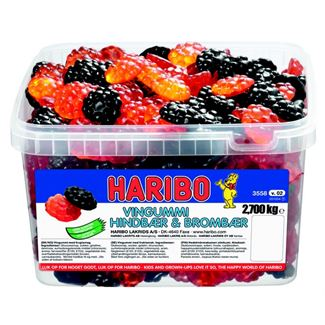
\includegraphics[scale=0.7]{fig/img/hindbaerbrombaer}
%
\captionof{figure}{$"$Vingummi hindbær og brumbær$"$-blanding fra Haribo.}
\label{mums}
\end{minipage}
%
\end{eks}

\subsubsection{1. Opskriv optimeringsproblemet på standardform med slack variabler.}
%
Generelt tager simplex modellen udgangspunkt i at alle variablerne er positive, og som beskrevet i afsnit \ref{sec:standard} så tilføjes $x_i^+$ og $x_i^-$, hvis der i optimeringsproblemet ikke er ikke-negativsbetingelser for variablen. 
I dette tilfælde er begge variabler positive og der er derfor ikke nødvendigt at opdele variablen. 
Med udgangspunkt i fremgangsmetoden fra afsnit \ref{sec:standard} så opstilles optimeringsproblemet derfor på standardform som
%
\begin{align*}
\begin{array}{lrrrrrlr}
\text{Maksimer}		& -5x_1 &-4x_2 &&& + z & =0\\
\text{begrænset af}	&3x_1& +5x_2	& + \textcolor{blue}{s_1} 	&&&= 	&78,\\
					&4x_1& + x_2	& & + \textcolor{blue}{s_2}	&&=	&	 36.\\
\end{array}
\end{align*}
%
Dog er maksimeringsproblemet omskrevet med udgangspunkt i 
\begin{align*}
-\textbf{c}^T\textbf{x} + z	 =0,
\end{align*}
hvor z er den optimale værdi. 
%
Slack-variablerne $s_1$ og $s_2$ er her markeret med blå, da de i sidste ende ikke tilføjes til løsningen. 
%
\subsubsection{2. Opstil simplex-tabllen for optimeringsproblemet}		
% 
Nu opstilles \textit{simplex-tabellen} for optimeringsproblemet. 
Med udgangspunkt i et generelt lineært optimeringsproblem på formen
%
% & =v, \text{ hvor } v=0
\begin{align*}
\begin{array}{lrl}
\text{Maksimér}		&-\textbf{c}^T\textbf{x} + z	& =0	\\
\text{begrænset af}	&A\textbf{x}	&=\mathbf{b},	\\
					&\mathbf{x}				&\geq \mathbf{0},
\end{array}
\end{align*}
er simplex-tabellen en matrix, som indeholder de lineære betingelser, slack-variablerne og objektfunktionen. 
Matrix $\mathbf{A}$ opskrives først, og derefter opskrives identitesmatricen $e_{m+1}$, hvor $m$ er lig mængden af slackvariabler samt den optimale løsning $z$, og til sidst opskrives $\mathbf{b}$. 
Under matrix $\mathbf{A}$ tilføjes matrix $- \mathbf{c}^T$. 
En generelt formel på simplex-tabellen med udgangspunkt i forrige optimeringsproblem ser dermed ud som følgende:
%
\begin{align*}
\begin{blockarray}{ccccccccccc}
x_1 & x_2 & \cdots & x_n & \textcolor{blue}{s_1} & \textcolor{blue}{s_2} &  \textcolor{blue}{\cdots} & \textcolor{blue}{s_m} & z & b \\
\begin{block}{[cccc|ccccc|c]c}
a_{1,1} & a_{1,2} & \cdots & a_{1,n} & 1 & 0 & \cdots & 0 & 0 & b_1 \\
a_{2,1} & a_{2,2} & \cdots & a_{2,n} & 0 & 1 & \cdots & 0 & 0 & b_2 \\
\vdots & \vdots & \ddots & \vdots & \vdots & \vdots & \ddots & \vdots & \vdots & \vdots \\
a_{m,1} & a_{m,2} & \cdots & a_{m,n} & 0 & 0 & \cdots  & 1  & 0 & b_{m}\\
\cline{1-10}
-c_1 & -c_2 & \cdots & -c_n & 0 & 0 & \cdots & 0 & 1 & v\\
\end{block}
\end{blockarray}.
\end{align*}
%
Optimeringsproblemet fra eksempel \ref{haribooooo} har dermed følgende simplex-tabel:
%
\begin{align*}
\begin{blockarray}{cccccc}
x_1 & x_2 & \textcolor{blue}{s_1} & \textcolor{blue}{s_2} & z & b \\
\begin{block}{[cc|ccc|c]}
3 & 5 & 1 & 0 & 0 & 78 \\
4 & 1 & 0 & 1 & 0 & 36 \\
\cline{1-6}
-5 & -4 & 0 & 0 & 1 & 0\\
\end{block}
\end{blockarray}.
\end{align*}
%
\subsubsection{3. Tjek optimering og identificer en pivotindgang}
%
Først tjekkes der efter optimering, og dette gøres ved at finde den største negative tal i objektfunktionen, altså nederste række i simplex-tabellen. 
Nedenstående er denne markeret:
%
\begin{align*}
\begin{blockarray}{cccccc}
x_1 & x_2 & \textcolor{blue}{s_1} & \textcolor{blue}{s_2} & z & b \\
\begin{block}{[cc|ccc|c]}
3 & 5 & 1 & 0 & 0 & 78 \\
4 & 1 & 0 & 1 & 0 & 36 \\
\cline{1-6}
\hlight{-5} & -4 & 0 & 0 & 1 & 0\\
\end{block}
\end{blockarray}.
\end{align*}
%
Søjlen, hvori denne værdi er, kaldes \textit{pivot-søjlen}. 
Herefter findes pivotindgangen og \textit{pivot-rækken}, ved at finde den mindste $x_i$-værdi ud fra 
\begin{align*}
\frac{a_{i,j}}{b_j}=x_i
\end{align*}
%
i pivot-søjlen.
For eksemplet findes pivotindgangen:
%
\begin{align*}
\frac{78}{3} =26 \text{  } \text{   } \frac{36}{4} =9.
\end{align*}
%
Eftersom $9$ er den laveste værdi er $4$ pivotindgangen og rækken den er i pivot-rækken. 
Nedenstående er pivotindgangen markeret:
%
\begin{align*}
\begin{blockarray}{cccccc}
x_1 & x_2 & \textcolor{blue}{s_1} & \textcolor{blue}{s_2} & z & b \\
\begin{block}{[cc|ccc|c]}
3 & 5 & 1 & 0 & 0 & 78 \\
\hlight{4} & 1 & 0 & 1 & 0 & 36 \\
\cline{1-6}
-5 & -4 & 0 & 0 & 1 & 0\\
\end{block}
\end{blockarray}.
\end{align*}	
%	
\subsubsection{4. Opstil en ny tabel ved hjælp af pivotering}
%
Med udgangspunkt i de elementære rækkeopperationer, se definition \ref{defn:element}, og Gauss-elimination, se afsnit \ref{gauss}, skaleres pivotindgangen til 1, og der skabes nuller under og over pivotindgangen ved hjælp af rækkeudskriftning.
Nedenstående ses dette gjort for eksemplet:
%
%& \begin{blockarray}{cccccc}
%x_1 & x_2 & \textcolor{blue}{s_1} & \textcolor{blue}{s_2} & z & b \\
%\begin{block}{[cc|ccc|c]}
%\hlight{3} & 5 & 1 & 0 & 0 & 78 \\
%4 & 1 & 0 & 1 & 0 & 36 \\
%\cline{1-6}
%\hlight{-5} & -4 & 0 & 0 & 1 & 0\\
%\end{block}
%\end{blockarray} \\
%
\begin{align*}
\xrightarrow[]{R_2 \rightarrow \frac{1}{4} R_2} &
\begin{blockarray}{cccccc}
x_1 & x_2 & \textcolor{blue}{s_1} & \textcolor{blue}{s_2} & z & b \\
\begin{block}{[cc|ccc|c]}
3 & 5 & 1 & 0 & 0 & 78 \\
1 & \frac{1}{4} & 0 & \frac{1}{4} & 0 & 9 \\
\cline{1-6}
-5 & -4 & 0 & 0 & 1 & 0\\
\end{block}
\end{blockarray} \\
\xrightarrow[R_3 \rightarrow R_3 + 5 R_2 ]{R_1 \rightarrow R_1 -3 R_2} &
\begin{blockarray}{cccccc}
x_1 & x_2 & \textcolor{blue}{s_1} & \textcolor{blue}{s_2} & z & b \\
\begin{block}{[cc|ccc|c]}
0 & \frac{17}{4} & 1 & \frac{-3}{4} & 0 & 51 \\
1 & \frac{1}{4} & 0 & \frac{1}{4} & 0 & 9 \\
\cline{1-6}
0 & \frac{-11}{4} & 0 & \frac{5}{4} & 1 & 45\\
\end{block}
\end{blockarray}.
\end{align*}	
%
\subsubsection{5. Kør 3 og 4 indtil den optimale løsning er fundet}
%
Denne proces forsættes nu indtil der ikke er flere negative tal i objektfunktionen.
\textit{Pivotering} er processen fra valget af den største negative værdi i objektfunktionen til at en ny værdi i objektfunktionen kan vælges. 
Der tjekkes derfor efter optimering igen, og en ny pivotindgang er valgt ved det største negative værdi. 
Denne er markeret i nedenstående matrix:	
%
\begin{align*}
\begin{blockarray}{cccccc}
x_1 & x_2 & \textcolor{blue}{s_1} & \textcolor{blue}{s_2} & z & b \\
\begin{block}{[cc|ccc|c]}
0 & \frac{17}{4} & 1 & \frac{-3}{4} & 0 & 51 \\
1 & \frac{1}{4} & 0 & \frac{1}{4} & 0 & 9 \\
\cline{1-6}
0 & \hlight{\frac{-11}{4}} & 0 & \frac{5}{4} & 1 & 45\\
\end{block}
\end{blockarray}
\end{align*}
%
Pivotindgangen findes ved:
%
\begin{align*}
\frac{51}{\frac{17}{4}} =12 \text{  } \text{   } \frac{9}{\frac{1}{4}} =36.
\end{align*}
%
Pivotindgangen er $\frac{17}{4}$ da denne giver den mindste værdi på $12$, hvilket er markeret i nedenstående matrix:
%
\begin{align*}
\begin{blockarray}{cccccc}
x_1 & x_2 & \textcolor{blue}{s_1} & \textcolor{blue}{s_2} & z & b \\
\begin{block}{[cc|ccc|c]}
0 & \hlight{\frac{17}{4}} & 1 & \frac{-3}{4} & 0 & 51 \\
1 & \frac{1}{4} & 0 & \frac{1}{4} & 0 & 9 \\
\cline{1-6}
0 & \frac{-11}{4} & 0 & \frac{5}{4} & 1 & 45\\
\end{block}
\end{blockarray}
\end{align*}
%
Pivotindgangen skaleres til 1, og der skabes nuller under og over pivotindgangen, ved de elementære regneregler:
%& \begin{blockarray}{cccccc}
%x_1 & x_2 & \textcolor{blue}{s_1} & \textcolor{blue}{s_2} &z & b \\
%\begin{block}{[cc|ccc|c]}
%0 & \frac{17}{4} & 1 & \frac{-3}{4} & 0 & 51 \\
%1 & \hlight{\frac{1}{4}} & 0 & \frac{1}{4} & 0 & 9 \\
%\cline{1-6}
%0 & \hlight{\frac{-11}{4}} & 0 & \frac{5}{4} & 1 & 45\\
%\end{block}
%\end{blockarray}\\
%
\begin{align*}
\xrightarrow[]{R_1 \rightarrow \frac{4}{17} R_1} &
\begin{blockarray}{cccccc}
x_1 & x_2 & \textcolor{blue}{s_1} & \textcolor{blue}{s_2} & z & b \\
\begin{block}{[cc|ccc|c]}
0 & 1 & \frac{4}{17} & \frac{-3}{17} & 0 & 12 \\
1 & \frac{1}{4} & 0 & \frac{1}{4} & 0 & 9 \\
\cline{1-6}
0 & \frac{-11}{4} & 0 & \frac{5}{4} & 1 & 45\\
\end{block}
\end{blockarray} \\
\xrightarrow[R_3 \rightarrow R_3 + \frac{11}{4} R_2 ]{R_2 \rightarrow R_2 -\frac{11}{4} R_1} &
\begin{blockarray}{cccccc}
x_1 & x_2 & \textcolor{blue}{s_1} & \textcolor{blue}{s_2} & z & b \\
\begin{block}{[cc|ccc|c]}
0 & 1 & \frac{4}{17} & \frac{-3}{17} & 0 & 12 \\
1 & 0 & \frac{-1}{17} & \frac{20}{17} & 0 & 6 \\
\cline{1-6}
0 & 0 & \frac{11}{17} & \frac{52}{17} & 1 & 78\\
\end{block}
\end{blockarray}.
\end{align*}	
%
%
\subsubsection{6. Identificer den optimale løsning}
%
Eftersom der ikke er flere negative værdier i objektfunktionen, er den optimale løsning nu fundet. 
Denne løsning, kan aflæses direkte af simplex-tabellen. 
Den optimale løsning for eksemplet er dermed:
%
\begin{align*}
x_1 & = 6, \\
x_2 & = 12, \\
z   & = 78.
\end{align*}
%